\chapter{积雪和土壤中水分的垂直运动}\label{积雪和土壤中水分的垂直运动}

\begin{mymdframed}{代码}
本章对应的代码文件为\texttt{MOD\_SoilSnowHydrology.F90}.
\end{mymdframed}

CoLM中地表的水分平衡分为无积雪和有积雪两种情形。

当无积雪时,
\begin{equation}
\Delta W_{ponding} = P_{rain}+S_{melt}+Q_{dew}-E-R-Q_{infl}
\end{equation}
其中$\Delta W_{ponding}$为地表积水的变化,$P_{rain}$为经过植被截留后到达地面的降水,$S_{melt}$为积雪融化后的水分,$Q_{dew}$为凝结的水分,$E$为土壤表面的蒸发,$R$为地表产流,$Q_{infl}$为入渗到土壤中的水分。

当有积雪时,
\begin{equation}
\Delta W_{ponding} = S_{melt}-R-Q_{infl}
\end{equation}
其中$\Delta W_{ponding}$为地表积水的变化,$S_{melt}$为由积雪空隙到达地表的液态水,$R$为地表产流,$Q_{infl}$为入渗到土壤中的水分。

积雪中的液态水平衡为,
\begin{equation}
\Delta W_{snow} = P_{rain}+Q_{dew}-S_{melt}-E
\end{equation}
其中$\Delta W_{snow}$为积雪空隙中液态水的变化,$P_{rain}$为经过植被截留后到达地面的降水,$Q_{dew}$为凝结的水分,$S_{melt}$为由积雪空隙到达地表的液态水,$E$为积雪表面的蒸发。

积雪中的液态水受毛细管力和重力的共同作用而流动,但由于毛细管力比重力小两个以上数量级,在计算的时候可以忽略。
水流通量一般表达为$K\times{\rm ss}^3$,其中$K$为导水率,${\rm ss}$为液态水在孔隙中的饱和度。由于没有有效的参数化方案来计算导水率$K$,
模式中采用简化的方案来近似液态水在积雪中的流动:当某一层中的液态水的含量超过了这一层的持水能力的时候,多余的液态水自这一层流入其下的一层。
某一层可保持的液态水的最大体积百分比计算为$ssi\cdot\left(1-v_{ice}\right)$,其中,$v_{ice}$为冰的体积百分比,$ssi$为束缚水饱和度,模式中取常数$ssi=0.033$。

土壤水的垂直运动受地表入渗、重力、土壤水吸力或压力以及植被吸水等过程的共同作用,CoLM中用Richards方程进行描述,
\begin{equation}
\frac{\partial \theta}{\partial t}=-\frac{\partial q}{\partial z}-S
\end{equation}
其中$z$为土壤深度,取土壤表面为0,垂直向下为正方向;$\theta$为土壤体积含水量,$q$为土壤水通量;$S$为源汇项,主要包含由植被水力过程和地下水的侧向运动引起的水分变化。

土壤水通量$q$在模式中用Buckingham-Darcy定律来描述,
\begin{equation}
q=-K \frac{\partial}{\partial z}(\psi-z)
\end{equation}
其中$\psi$为土壤水势,$K$为土壤导水率。

为了使Richards方程闭合,需使用土壤水含量$\theta$,土壤水势$\psi$和土壤导水率$K$三者之间关系的经验公式,称为土壤水力特征曲线。CoLM中可使用~\citet{campbell1974} 和~\citet{van1980closed} 建立的两种土壤水力特征曲线。

\citet{campbell1974}建立的曲线为,
\begin{equation}\label{eq:SW_CB}
\psi=\psi_{s}\left(\frac{\theta}{\theta_{sat}}\right)^{-B}
\end{equation}
\begin{equation}\label{eq:Ks_CB}
K=K_{s}\left(\frac{\theta}{\theta_{s}}\right)^{2 B+3}
\end{equation}
其中$\psi_s$为饱和土水势,$\theta_{s}$为饱和土壤体积含水量,$K_{s}$为饱和导水率,$B$为曲线参数。

\citet{van1980closed} 建立的曲线为
\begin{equation}\label{eq:SW_VG}
    \Theta = \frac{\theta-\theta_r}{\theta_s-\theta_r} = \left[\frac{1}{1+\left(\alpha h\right)^n}\right]^{1-1/n}
\end{equation}
\begin{equation}\label{eq:Ks_VG}
    K = K_s \Theta^L \left[1-\left(1-\Theta^{1/\left(1-1/n\right)}\right)^{1-1/n}\right]^2
\end{equation}
其中$h$为土壤吸力势,$\theta_r$为残余含水量,$\theta_s$为饱和含水量,$K_{s}$为饱和导水率,$\alpha$、$L$ 和 $n$为曲线参数。

CoLM中可选两个数值方案进行Richards方程的求解:1. 2014版CoLM中的方案;2. 可变饱和流算法。

\section{2014版Richards方程求解方案}

{
\begin{figure}[htbp]
\centering
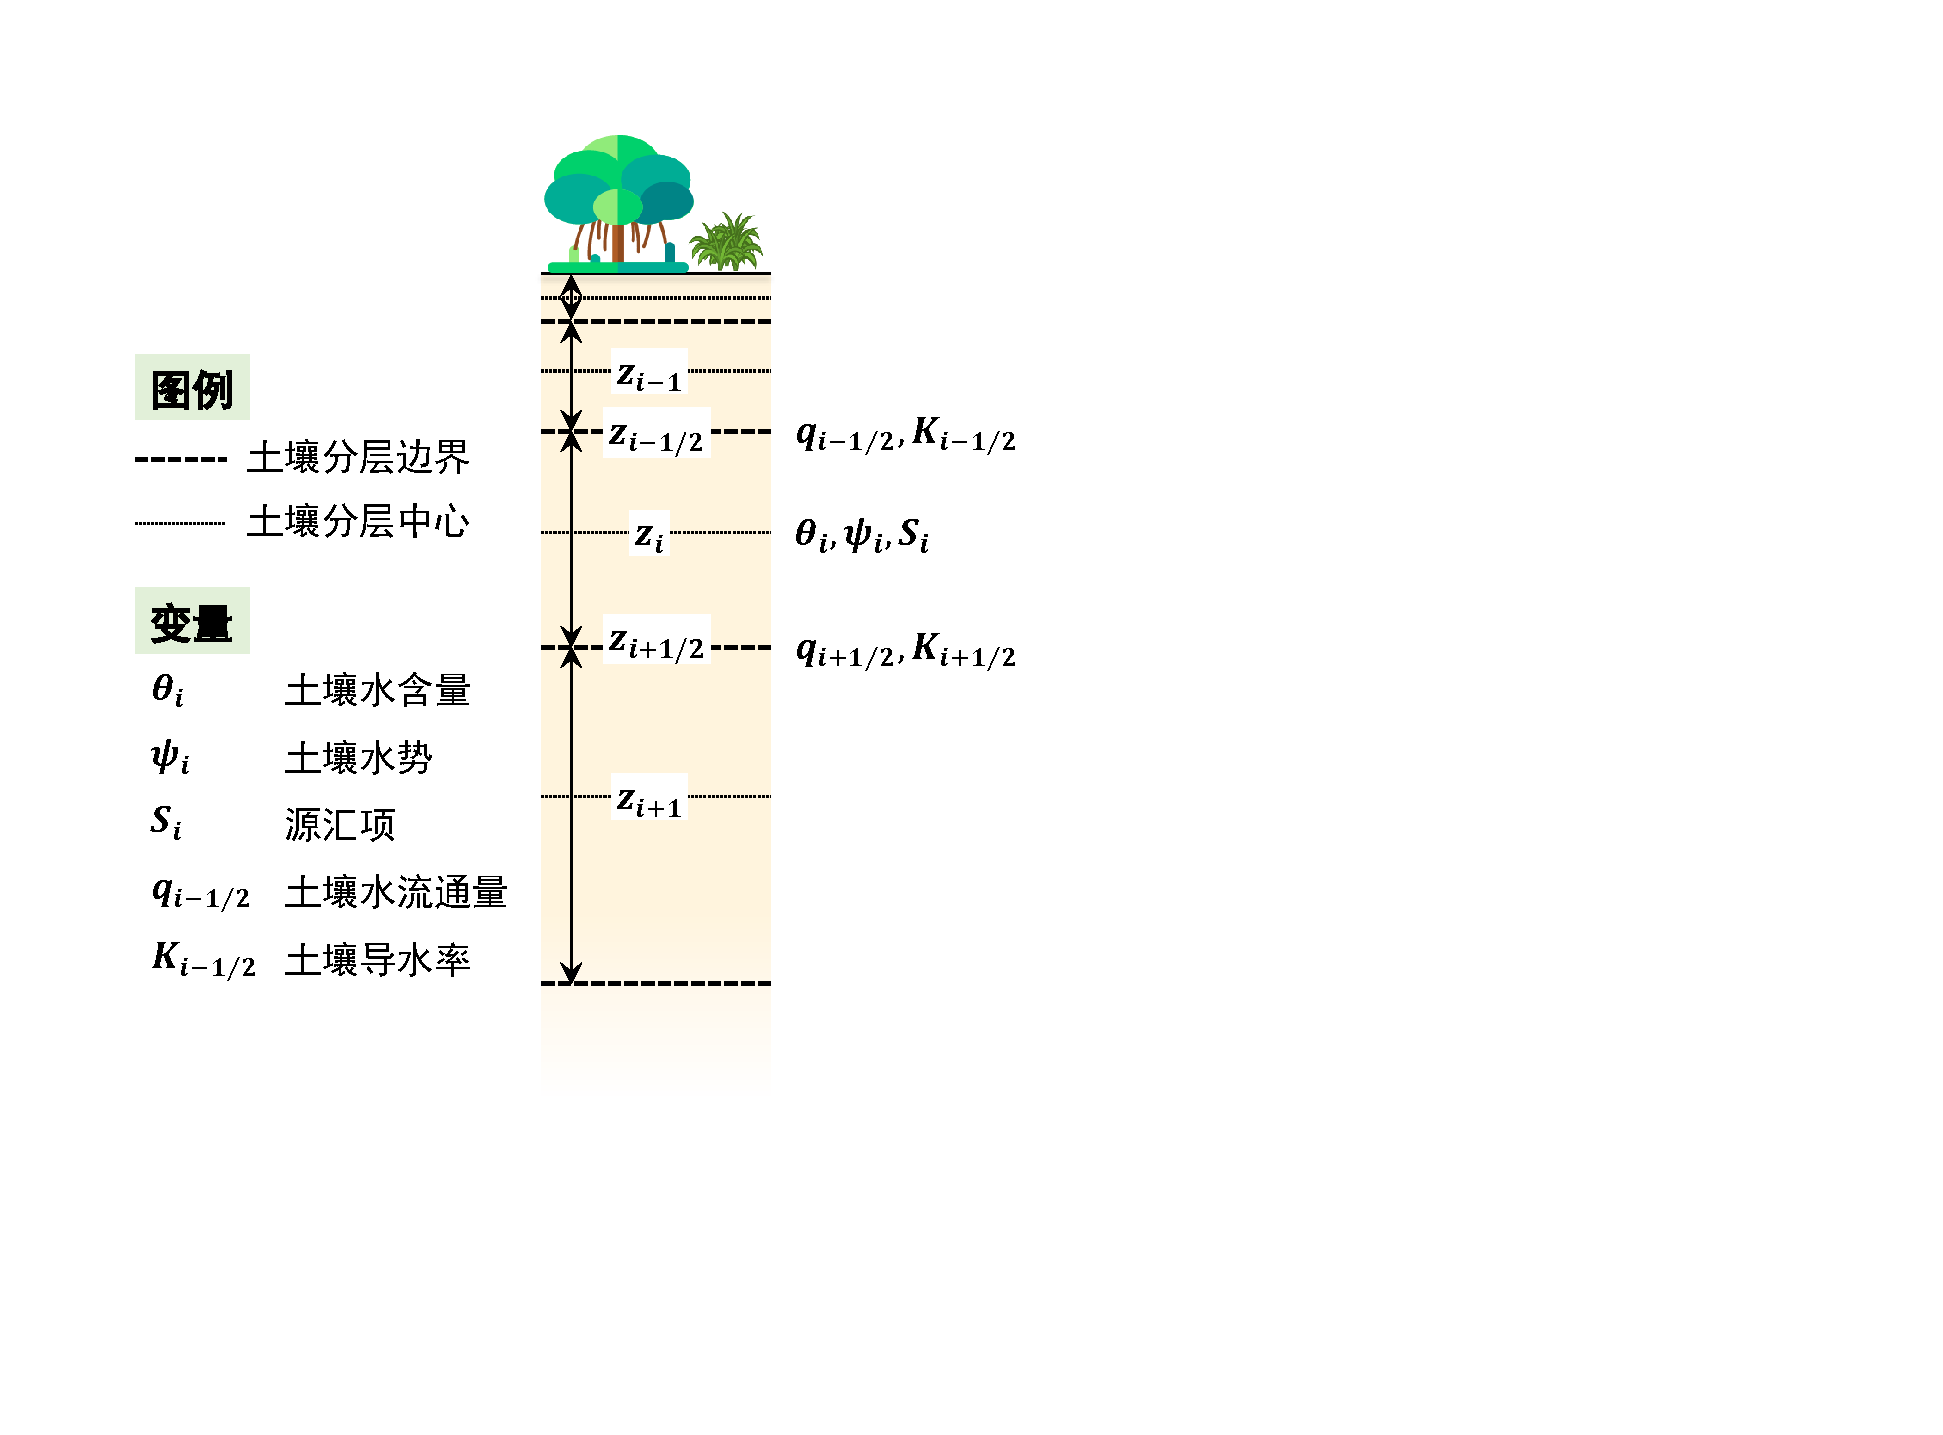
\includegraphics[width=0.8\textwidth]{Figures/植被冠层和土壤水分/土壤水离散.pdf}
\caption{离散Richards方程中各项的定义}
\label{fig:土壤水离散}
\end{figure}
}

\subsection{基于土壤湿度的Richards方程求解方案}

首先建立离散的Richards方程。土壤的具体分层方案见章节~\ref{土壤和积雪的垂直分层},离散后变量的定义见示意图~\ref{fig:土壤水离散}。在第$i$层上,对Richards方程进行空间上的积分可得
\begin{equation}
\Delta z_{i} \frac{\partial}{\partial t} \theta_{i}=-\left(q_{i+\frac{1}{2}}-q_{i-\frac{1}{2}}\right)-S_{i}
\end{equation}
\begin{equation}
q_{i+\frac{1}{2}}=-K_{i+\frac{1}{2}}\left(\frac{\psi_{i+1}-\psi_{i}}{\Delta z_{i+\frac{1}{2}}}-1\right)
\end{equation}
其中$\Delta {z_i}$为第$i$层的厚度,$\theta_i$为第$i$层的平均土壤含水量,
$q_{i+\frac{1}{2}}$为第$i$层和第$i+1$层之间的土壤水通量,$K_{i+\frac{1}{2}}$为第$i$层和第$i+1$层之间的等效导水率,$\Delta z_{i+\frac{1}{2}}$表示从第$i$层到第$i+1$层中心的距离,$S_i$为第$i$层内的源汇项。在时间上采用隐格式,可得
\begin{equation}
\Delta z_{i} \frac{\theta_{i}^{n+1}-\theta_{i}^{n}}{\Delta t}=-\left(q_{i+\frac{1}{2}}^{n+1}-q_{i-\frac{1}{2}}^{n+1}\right)-S_{i}
\end{equation}
\begin{equation}
q_{i+\frac{1}{2}}^{n+1}=-K_{i+\frac{1}{2}}^{n+1}\left(\frac{\psi_{i+1}^{n+1}-\psi_{i}^{n+1}}{\Delta z_{i+\frac{1}{2}}}-1\right)
\end{equation}
为了简化计算,将$q_{i+\frac{1}{2}}^{n+1}$表达式中的各项在$\theta_i^n$附近做一阶近似,可得
\begin{equation}
\begin{aligned}
K_{i+\frac{1}{2}}^{n+1} &\approx K_{i+\frac{1}{2}}^{n}+\frac{\partial K_{i+\frac{1}{2}}}
    {\partial \theta_{i}}\left(\theta_{i}^{n+1}-\theta_{i}^{n}\right)+\frac{\partial K_{i+\frac{1}{2}}}
    {\partial \theta_{i+1}}\left(\theta_{i+1}^{n+1}-\theta_{i+1}^{n}\right) \\ 
\psi_{i+1}^{n+1} &\approx \psi_{i+1}^{n}+\frac{\partial \psi_{i+1}}{\partial \theta_{i+1}}\left(\theta_{i+1}^{n+1}-\theta_{i+1}^{n}\right) \\
\psi_{i}^{n+1} &\approx \psi_{i}^{n}+\frac{\partial \psi_{i}}{\partial \theta_{i}}\left(\theta_{i}^{n+1}-\theta_{i}^{n}\right)
\end{aligned}
\end{equation}

记$\Delta \theta_i=\theta_i^{n+1}-\theta_i^n$,则
\begin{equation}
\begin{split} 
q_{i+\frac{1}{2}}^{n+1} \approx &-\left(K_{i+\frac{1}{2}}^{n}+\frac{\partial K_{i+\frac{1}{2}}}{\partial \theta_{i}} \Delta \theta_{i} + \frac{\partial K_{i+\frac{1}{2}}}{\partial \theta_{i+1}} \Delta \theta_{i+1}\right)  \\
    & \times \left[\frac{1}{\Delta z_{i+\frac{1}{2}}}\left(\psi_{i+1}^{n}+\frac{\partial \psi_{i+1}}{\partial \theta_{i+1}} \Delta \theta_{i+1}-\psi_{i}^{n}-\frac{\partial \psi_{i}}
    {\partial \theta_{i}} \Delta \theta_{i}\right)-1\right] \\ 
    \approx & -K_{i+\frac{1}{2}}^{n}\left[\frac{1}{\Delta z_{i+\frac{1}{2}}}\left(\psi_{i+1}^{n}-\psi_{i}^{n}\right)-1\right] \\
    &-\left[-K_{i+\frac{1}{2}}^{n} \frac{1}{\Delta z_{i+\frac{1}{2}}} \frac{\partial \psi_{i}}{\partial \theta_{i}}+\frac{\partial K_{i+\frac{1}{2}}}{\partial 
     \theta_{i}}\left(\frac{1}{\Delta z_{i+\frac{1}{2}}}\left(\psi_{i+1}^{n}-\psi_{i}^{n}\right)-1\right)\right] \Delta \theta_{i} \\ 
    &-\left[K_{i+\frac{1}{2}}^{n} \frac{1}{\Delta z_{i+\frac{1}{2}}} \frac{\partial \psi_{i+1}}{\partial \theta_{i+1}}+\frac{\partial K_{i+\frac{1}{2}}}{\partial
      \theta_{i+1}}\left(\frac{1}{\Delta z_{i+\frac{1}{2}}}\left(\psi_{i+1}^{n}-\psi_{i}^{n}\right)-1\right)\right] \Delta \theta_{i+1} 
\end{split}
\end{equation}
其中第一个约等号是对各项做一阶近似,第二个约等号是舍弃二阶项。对$q_{i-\frac{1}{2}}^{n+1}$也可做同样的近似。从而,完全离散后的Richards方程可表达为,
\begin{equation}
a_i \Delta \theta_{i-1}+b_i \Delta \theta_{i}+c_i \Delta \theta_{i+1}=r_i
\end{equation}
其中,
\begin{equation}
\begin{aligned}
 a_i &= - K_{i-\frac{1}{2}}^{n} \frac{1}{\Delta z_{i-\frac{1}{2}}}
     \frac{\partial \psi_{i-1}}{\partial \theta_{i-1}}+\frac{\partial K_{i-\frac{1}{2}}}
     {\partial \theta_{i-1}}\left(\frac{1}{\Delta z_{i-\frac{1}{2}}}\left(\psi_{i}^{n}-\psi_{i-1}^{n}\right)-1\right) \\
b_i &= \frac{\Delta z_{i}}{\Delta t}+K_{i+\frac{1}{2}}^{n} \frac{1}{\Delta z_{i+\frac{1}{2}}} 
      \frac{\partial \psi_{i}}{\partial \theta_{i}}-\frac{\partial K_{i+\frac{1}{2}}}{\partial \theta_{i}}
      \left(\frac{1}{\Delta z_{i+\frac{1}{2}}}\left(\psi_{i+1}^{n}-\psi_{i}^{n}\right)-1\right) \\
&\mathrel{\phantom{=}}+K_{i-\frac{1}{2}}^{n} \frac{1}{\Delta z_{i-\frac{1}{2}}} \frac{\partial \psi_{i}}{\partial 
       \theta_{i}}+\frac{\partial K_{i-\frac{1}{2}}}{\partial \theta_{i}}\left(\frac{1}{\Delta z_{i-\frac{1}{2}}}\left(\psi_{i}^{n}-\psi_{i-1}^{n}\right)-1\right) \\ 
c_i &= - K_{i+\frac{1}{2}}^{n} \frac{1}{\Delta z_{i+\frac{1}{2}}} 
       \frac{\partial \psi_{i+1}}{\partial \theta_{i+1}} - \frac{\partial K_{i+\frac{1}{2}}}{\partial \theta_{i+1}}\left(\frac{1}
       {\Delta z_{i+\frac{1}{2}}}\left(\psi_{i+1}^{n}-\psi_{i}^{n}\right)-1\right) \\ 
r_i &= K_{i+\frac{1}{2}}^{n}
       \left(\frac{1}{\Delta z_{i+\frac{1}{2}}}\left(\psi_{i+1}^{n}-\psi_{i}^{n}\right)-1\right)-K_{i-\frac{1}{2}}^{n}
       \left(\frac{1}{\Delta z_{i-\frac{1}{2}}}\left(\psi_{i}^{n}-\psi_{i-1}^{n}\right)-1\right)-S_{i}
\end{aligned}
\end{equation}

对最上面的土壤分层(第1层),使用给定的入渗通量$Q_{infl}$,则
\begin{equation}
\begin{aligned}
a_1 &= 0 \\
b_1 &= \frac{\Delta z_1}{\Delta t}+K_{1+\frac{1}{2}}^{n} 
    \frac{1}{\Delta z_{1+\frac{1}{2}}} \frac{\partial \psi_{1}}{\partial \theta_{1}}-\frac{\partial K_{1+\frac{1}{2}}}{\partial \theta_{1}}\left(\frac{1}{\Delta z_{1+\frac{1}{2}}}
    \left(\psi_{2}^{n}-\psi_{1}^{n}\right)-1\right) \\
c_1 &= -K_{1+\frac{1}{2}}^{n} \frac{1}{\Delta z_{1+\frac{1}{2}}} 
    \frac{\partial \psi_{2}}{\partial \theta_{2}}-\frac{\partial K_{1+\frac{1}{2}}}{\partial \theta_{2}}\left(\frac{1}{\Delta z_{1+\frac{1}{2}}}
    \left(\psi_{2}^{n}-\psi_{1}^{n}\right)-1\right) \\ 
r_1 &= Q_{infl}+K_{1+\frac{1}{2}}^{n}
    \left(\frac{1}{\Delta z_{1+\frac{1}{2}}}\left(\psi_{2}^{n}-\psi_{1}^{n}\right)-1\right)-S_{1}
\end{aligned}
\end{equation}

对最下面的土壤分层(第$I$层),假定边界条件为重力排水边界条件,即$q_{I+\frac{1}{2}}^{n+1}=K_{I}^{n+1}$,则
\begin{equation}
\begin{aligned}
a_I &= - K_{I-\frac{1}{2}}^{n} \frac{1}{\Delta z_{I-\frac{1}{2}}}
     \frac{\partial \psi_{I-1}}{\partial \theta_{I-1}}+\frac{\partial K_{I-\frac{1}{2}}}
     {\partial \theta_{I-1}}\left(\frac{1}{\Delta z_{I-\frac{1}{2}}}\left(\psi_{I}^{n}-\psi_{I-1}^{n}\right)-1\right) \\
b_I &= \frac{\Delta z_{I}}{\Delta t}+\frac{\partial K_{I}}
    {\partial \theta_{I}}+K_{I-\frac{1}{2}}^{n} \frac{1}{\Delta z_{I-\frac{1}{2}}} \frac{\partial \psi_{I}}{\partial \theta_{I}}+
    \frac{\partial K_{I-\frac{1}{2}}}{\partial \theta_{I}}\left(\frac{1}{\Delta z_{I-\frac{1}{2}}}\left(\psi_{I}^{n}-\psi_{I-1}^{n}\right)-1\right) \\
c_I &= 0 \\
r_I &= -K_{I}^{n}-K_{I-\frac{1}{2}}^{n}\left(\frac{1}{\Delta z_{I-\frac{1}{2}}}\left(\psi_{I}^{n}-\psi_{I-1}^{n}\right)-1\right)-S_{I}
\end{aligned}
\end{equation}

求解上述方程组,即可得到土壤水含量的变化量。方程组的系数矩阵为三对角阵,矩阵中各项均定义在第$n$步,可显式计算出,所得代数方程组可用追赶法快速求解。

在2014版Richards方程求解方案中,仅使用~\citet{campbell1974}建立的土壤水力特征曲线。$K_{i+\frac{1}{2}}$是两层土壤土壤之间的等效导水率,若采用上游格式,其定义为
\begin{equation}
    K_{i+\frac{1}{2}}=
    \begin{cases}
       K_{s,i}\left(\frac{\theta_{i}}{\theta_{s,i}}\right)^{2 B_i+3}
       & q_{i+\frac{1}{2}} \geqslant 0 \quad \mbox{(水流方向向下)}\\ 
       K_{s,i+1}\left(\frac{\theta_{i+1}}{\theta_{s,i+1}}\right)^{2 B_{i+1}+3}
       & q_{i+\frac{1}{2}} < 0 \quad \mbox{(水流方向向上)}
    \end{cases}
\end{equation}
在系数矩阵中,需要对土壤水势和等效导水率求导数。对土壤水势,容易计算得到
\begin{equation}
\frac{\partial \psi_{i}}{\partial \theta_{i}}=-B_i \frac{\psi_{i}}{\theta_{i}}
\end{equation}
对等效导水率,则导数为
\begin{align}
\frac{\partial K_{i+\frac{1}{2}}}{\partial \theta_{i}} & = 
\begin{cases}
  \left(2B_i+3\right) K_{s,i}\left(\frac{\theta_{i}}{\theta_{s,i}}\right)^{2B_i+2} 
    \frac{1}{\theta_{s,i}}, & q_{i+\frac{1}{2}} \geqslant 0 \\ 
   0, & q_{i+\frac{1}{2}} < 0 
  \end{cases}
\\
\frac{\partial K_{i+\frac{1}{2}}}{\partial \theta_{i+1}} & = 
\begin{cases}
     0, & q_{i+\frac{1}{2}} \geqslant 0 \\
     (2B_{i+1}+3) K_{s,i+1}\left(\frac{\theta_{i+1}}{\theta_{s,i+1}}\right)^{2B_{i+1}+2} \frac{1}{\theta_{ {s,i+1}}}, & q_{i+\frac{1}{2}} < 0 
   \end{cases}
\end{align}
对计算区域的底部(第$I$层),
\begin{equation}
K_{I}=K_{s,I}\left(\frac{\theta_{I}}{\theta_{s,I}}\right)^{2B_I+3}, \quad \frac{\partial K_{I}}
{\partial \theta_{I}} = (2B_I+3) K_{s,I}\left(\frac{\theta_{I}}{\theta_{s,I}}\right)^{2B_I+2} \frac{1}{\theta_{s,I}}
\end{equation}

有冰存在的时候,需考虑冰对导水率的影响,使用如下经验公式,
\begin{equation}
    {f}_{imped,i+\frac{1}{2}}=10^{-e_{ice}\cdot\frac{f_{ice, i}+f_{ice, i+1}}{2}}
\end{equation}
其中$e_{ice}=6.0$为冰的阻抗因子。对等效导水率及其导数的限制为
\begin{equation}
\begin{aligned}
K_{i+\frac{1}{2}} & = {f}_{imped,i+\frac{1}{2}} \cdot K_{i+\frac{1}{2}} \\ 
\frac{\partial K_{i+\frac{1}{2}}}{\partial \theta_{i}}
    & = {f}_{imped,i+\frac{1}{2}} \cdot \frac{\partial K_{i+\frac{1}{2}}}{\partial \theta_{i}} \\ 
\frac{\partial K_{i+\frac{1}{2}}}{\partial \theta_{i+1}} & =
    {f}_{imped,i+\frac{1}{2}} \cdot \frac{\partial K_{i+\frac{1}{2}}}{\partial \theta_{i+1}}
    \end{aligned}
\end{equation}

\subsection{饱和含水层}
模式中使用两个变量$w_a$和$z_{wt}$来描述饱和含水层的状态,分别代表总水量和地下水位。饱和含水层中的水分可与土壤层中的水分在垂直方向进行交换,也可在水平方向进行流动。其中水平方向的流动被称为地下径流,相关内容见第六部分水文过程。

土壤层与饱和含水层的交换通量定义为土壤层底部的水流通量,
\begin{equation}
{q}_{recharge}=q_{I+\frac{1}{2}}^{n+1}=K_{I}^{n+1} = K_I^n + \frac{\partial K_{I}}{\partial \theta_{I}} \Delta \theta_{I}
\end{equation}

含水层总水量变化为
\begin{equation}
w_{a}=w_{a}+q_{recharge} \cdot \Delta t
\end{equation}

给水度$S_y$(specific yield)反映了含水层水量变化时地下水位的变化。假设地下水位之上的土壤为均质土壤,且土壤水处于平衡态,则其土壤水势可表达为深度的函数,
\begin{equation}
    \psi \left(z\right) = \psi_s - \left(z_{wt} - z\right)
\end{equation}
地下水位之上的土壤中所含水分的总量为
\begin{equation}
    w_{unsat} = \int^{z_{wt}}_0 \theta\left[\psi\left(z\right)\right] \mathrm{d}z = \int^{z_{wt}}_0 \theta\left[\psi_s - \left(z_{wt} - z\right)\right] \mathrm{d}z
\end{equation}
使用~\citet{campbell1974}建立的土壤水力特征曲线时,
\begin{equation}
    w_{unsat} = \int^{z_{wt}}_0 \theta_s\left[\frac{\psi_s - \left(z_{wt} - z\right)}{\psi_s}\right]^{-\frac{1}{B}} \mathrm{d}z
\end{equation}
假设饱和含水层最大到$z_{max}$,则地下水位之下的水分总量为
\begin{equation}
w_{sat} = \theta_s\left(z_{max}-z_{wt}\right)
\end{equation}
土壤$0$到$z_{max}$深度的总水量为
\begin{equation}
    w_{total} = w_{unsat} + w_{sat} = \int^{z_{wt}}_0 \theta_s\left[\frac{\psi_s - \left(z_{wt} - z\right)}{\psi_s}\right]^{-\frac{1}{B}} \mathrm{d}z + \theta_s\left(z_{max}-z_{wt}\right)
\end{equation}
对$z_{wt}$求导数可得给水度$S_y$,
\begin{equation}
{S}_{{y}} = -\frac{w_{total}}{z_{wt}} = \theta_{s}\left[1-\left(1-\frac{z_{w t}}{\psi_{s}}\right)^{-\frac{1}{B}}\right] \label{eqn:s_y}
\end{equation}
这里取符号是因为深度的正方向向下,总水量越多,则地下水位越浅。不难发现,$S_y$等于地下水位位于$z_{wt}$且土壤水处于平衡状态时,土壤表层($z=0$)的空气体积含量百分比,这是因为在平衡态的假设下,水分的增加会使得含水量曲线整体向上移动,等效于最上层干旱部分被地下水位附近的饱和部分取代。

若地下水位位于最下层土壤之下,公式(\ref{eqn:s_y})中的参数$\theta_s$、$\psi_s$ 和 $B$取最下层土壤的值,则水位的变化为
\begin{equation}
z_{w t}=z_{w t}-\frac{q_{recharge} \cdot \Delta t}{s_{y}}
\end{equation}

若地下水位位于分层土壤之内,则需要逐层计算水位的变化。当$q_{recharge}>0$时,记地下水位所在层为$j$,
\begin{equation}
{S}_{y,j}=\theta_{s,j}\left[1-\left(1-\frac{z_{wt}}{\psi_{s,j}}\right)^{-\frac{1}{B_j}}\right]
\end{equation}
在第$j$层可容纳水量的限制下,实际可补给到第$j$层的水量为($z_{j-\frac{1}{2}}$为第$j$层的上边界)
\begin{equation}
q_{recharge, i}=\min \left(q_{recharge}, \frac{S_{y,j} \cdot \left(z_{w t}-z_{i-\frac{1}{2}}\right)}{\Delta t} \right)  
\end{equation}
地下水位在第$j$层内的变化为
\begin{equation}
z_{w t}=z_{w t}-\frac{q_{recharge,j} \cdot \Delta t}{S_{y,j}}
\end{equation}
若$q_{recharge,j}<q_{recharge}$,则此时地下水位上升至第$j-1$层,补给水未用尽,可继续对第$j-1$层进行补给,直至补给水用尽或者到达土壤表面。

当$q_{recharge}<0$时,水分从饱和含水层向上层土壤进行补给,$w_a$减少,$z_{wt}$增加,除方向相反外,计算过程与从上层土壤向饱和含水层的补给类似,这里不再赘述。

\section{可变饱和流数值算法}

\begin{mymdframed}{代码}
本节对应的代码文件为\texttt{HYDRO/MOD\_Hydro\_SoilWater.F90}.
\end{mymdframed}

可变饱和流数值算法(Variably Saturated Flow, VSF)\citep{dai2019vsf}在多个方面对Richards方程的数值算法进行了改进。

{
\begin{figure}[htbp]
\centering
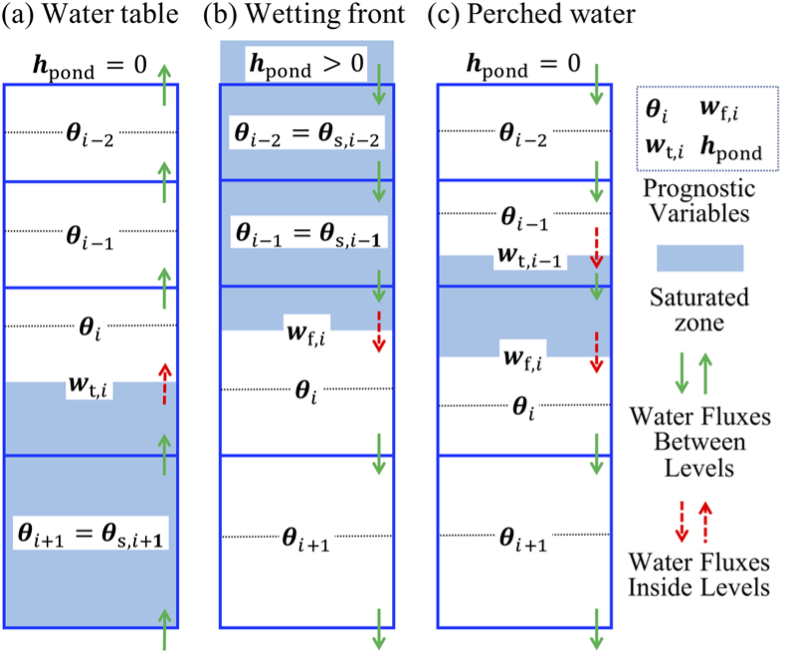
\includegraphics{Figures/陆地表面的水分循环/可变饱和流数值算法预报区域空间结构示意图.png}
\caption{可变饱和流数值算法空间离散方法示意图}
\label{fig:可变饱和流数值算法预报区域空间结构示意图}
\end{figure}
}

首先,引入了两个新的预报变量(地下水位,湿润锋面的位置)来追踪饱和区的边界(图 \ref{fig:可变饱和流数值算法预报区域空间结构示意图})。借助于这两个新的预报变量,在非饱和区,Richards方程具有类似抛物型方程的性质,将含水量作为主要预报变量;而在饱和区,Richards方程具有类似椭圆型方程的性质,仅需确定区域边界上的水势压力便可求解区域内部均一的水流通量。这一方法属于“土壤水势-含水量”混合形式Richards方程的范畴,但相比传统的混合形式Richards方程,能更清晰地刻画土壤水运动在不同区域内的物理和数学性质。

其次,可变饱和流算法使用了一个新的土壤层间等效导水率计算公式。与常用的简单导水率计算公式相比,新公式具有更高的精度。新计算公式与隐式时间积分格式结合,可导出理论上无数值振荡的离散格式,提高了数值解的稳定性。

再者,可变饱和流算法使用了混合隐式-显式时间积分方案和自适应时间步长。隐式时间积分的求解需要在单步内进行迭代,当迭代算法失效或者时间步长较小时,使用一个满足质量守恒的显式积分格式进行替代。自适应时间步长可在精度和效率之间做出合理的平衡。

最后,可变饱和流数值算法将地表入渗、土壤水运动和土壤水与地下水的相互交换这三个垂直方向的水流运动进行统一求解。侧向的地表水运动(坡面流)将地表水深作为预报变量,侧向的地下水运动(基流)将地下水位作为预报变量,在模拟土壤水运动时,也使用了这两个变量,实现了垂直方向和水平方向的变量统一,使陆面模型在物理上更协调。


\subsection{土壤水预报方程}
在每个土壤层内,可使用三个预报变量来描述土壤中液态水的分布情况。
土壤体积含水量为固定的预报变量($\theta_i$)。为了追踪土壤中饱和水层的变化(包括地下水、滞水层和入渗情况下由地表向下发展的饱和水层),
每层土壤中引入了另外两个潜在的预报变量($w_{f,i}$和$w_{t,i}$),
分别代表土壤层内上部饱和区域的厚度,和土壤层内下部饱和区域的厚度(图~\ref{fig:可变饱和流数值算法预报区域空间结构示意图}),
当某层土壤部分饱和时,这两个变量被激活。
{
\begin{figure}[htbp]
\centering
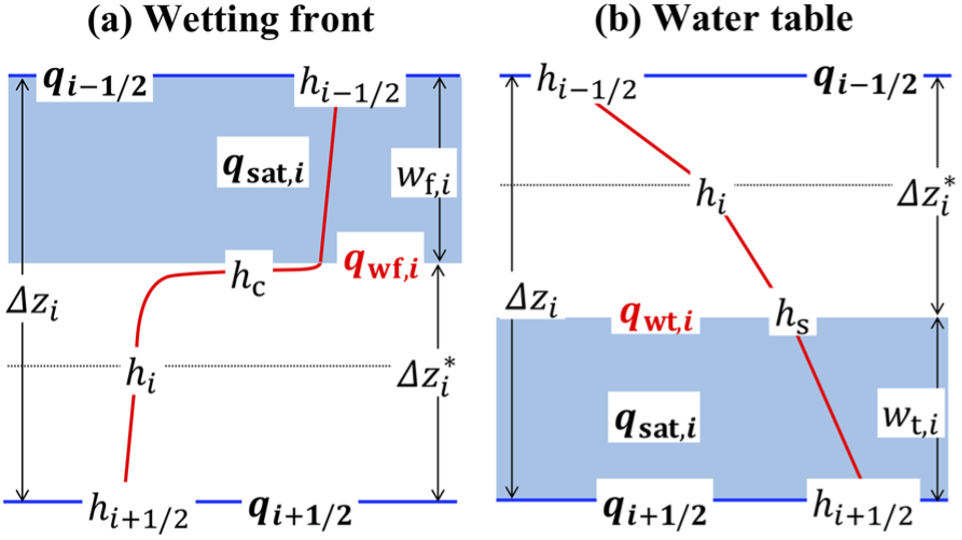
\includegraphics{Figures/陆地表面的水分循环/饱和-非饱和过渡状态的土壤层.png}
\caption[饱和-非饱和过渡状态的土壤层]{饱和-非饱和过渡状态的土壤层。如果土壤层内上部有饱和区(左图),
层内饱和区的厚度作为预报变量被激活;如果土壤层内下部有饱和区(右图),层内饱和区的厚度作为预报变量被激活}
\label{fig:饱和-非饱和过渡状态的土壤层}
\end{figure}
}

预报变量$\theta_i$的预报方程为
\begin{equation}\label{si_in1}
\left(\Delta z_{i}-w_{f, i}^{n+1}-w_{t, i}^{n+1}\right) \cdot\left(\theta_{i}^{n+1}-\theta_{i}^{n}\right)=\Delta t \cdot\left(q_{ {uin,i }}^{n+1}-q_{uout,i}^{n+1}\right)
\end{equation}
其中,$\Delta z_i$ 为第$ i $层土壤的厚度,$\Delta t$ 为时间步长,$q_{uin,i}^{n+1}$为非饱和区域上边界处的水流通量,$q_{uout,i}^{n+1}$为非饱和区域下边界处的水流通量。


预报变量$w_{f,i}$表示土壤层上部饱和区域的厚度,其预报方程为
\begin{equation}\label{si_in2}
\left(\theta_{s, i}-\theta_{i}^{n}\right) \cdot\left(w_{f, i}^{n+1}-w_{f, i}^{n}\right)=\Delta t \cdot\left(q_{i-1/2}^{n+1}-q_{w f, i}^{n+1}\right)
\end{equation}
其中,$\theta_{s,i}$ 为第$ i$ 层土壤的饱和体积含水量,$ q_{{i-1/2}}^{n+1}$为第$i$层土壤上边界处的水流通量,$q_{wf,i}^{n+1}$为饱和区域下边界处(湿润锋面)的水流通量。


预报变量$w_{t,i}$表示土壤层下部饱和区域的厚度,其预报方程为
\begin{equation}\label{si_in3}
\left(\theta_{s, i}-\theta_{i}^{n}\right) \cdot\left(w_{t, i}^{n+1}-w_{t, i}^{n}\right)=\Delta t \cdot\left(q_{w t, i}^{n+1}-q_{i+1 / 2}^{n+1}\right)
\end{equation}
其中,$q_{wt,i}^{n+1}$  为饱和区域上边界处的水流通量,$q_{i+1/2}^{n+1}$为第$i$层土壤下边界处的水流通量。

% 在未饱和的土壤层,模式使用预报方程(\ref{si_in1})预报体积含水量的变化;
% 若未饱和的土壤层内上部有饱和区域,模式联合预报方程(\ref{si_in1})和(\ref{si_in2})来同时预报饱和区域的边界变化和非饱和区域内土壤积水含水量的变化;
% 若未饱和的土壤层内下部有饱和区域,模式联合预报方程(\ref{si_in1})和(\ref{si_in3})来同时预报饱和区域的边界变化和非饱和区域内土壤积水含水量的变化;
% 若未饱和的土壤层内上下部分均有饱和区域,模式联合预报方程(\ref{si_in1})--(\ref{si_in3})来同时预报饱和区域的边界变化和非饱和区域内土壤积水含水量的变化。

% 在地下部分,所有未饱和土壤层内的上述预报方程联合在一起组成一个方程组,来进行统一求解。

\subsection{地表积水的变化}
为了预报由入渗所产生的地表水深的变化,地表积水深度($h_{pond}$)也是算法中的预报变量,其预报方程为
\begin{equation}\label{hpond}
h_{ {pond }}^{n+1}-h_{ {pond }}^{n}=\Delta t \cdot\left(q_{ {surf }}^{n+1}-q_{ {infl }}^{n+1}\right)
\end{equation}
其中,$q_{surf}^{n+1} $ 为从地表水上部进入的水流通量,
其可以是降水、蒸发、或者地表水与积雪的液态水交换;$q_{infl}^{n+1}$为从地表进入土壤的水流通量。


当地表有积水,或者由于进入地表的水流通量大于入渗到土壤中的通量而形成积水时,积水深度的预报方程(\ref{hpond})也加入到土壤水的方程组中,进行统一求解。


\subsection{地下水的变化}
当地下水位在土壤水计算区域内部时,其位置由$w_{t,i}$进行预报。

当地下水位处于土壤水计算区域之下时,使用预报变量$W_a$来表示计算区域之下蓄水层的蓄水状态。$W_a$定义为
\begin{equation}
W_{a}=-\int_{z_{b t m}}^{Z_{w t}}\left(\theta_{s}-\theta\right) d z
\end{equation}
$W_a$的绝对值为土壤水计算区域之下空气的体积百分比,负号的含义是计算区域之下液态水相对于饱和状态是亏缺的,$W_a$的最大值为0(表示土壤水饱和)。


$W_a$的预报方程为
\begin{equation}\label{wa_n1_n}
W_{a}^{n+1}-W_{a}^{n}=\Delta t \cdot q_{b t m}^{n+1}
\end{equation}
当地下水位处于土壤水计算区域之下时,$W_a$的预报方程(\ref{wa_n1_n})也加入到土壤水的方程组中,进行统一求解。

\subsection{水流通量的计算}
预报方程(\ref{si_in1})--(\ref{wa_n1_n})中,右端项中均包含了水流通量的计算,其计算分为以下几种情形,
\begin{enumerate}
    \item 饱和区域内部的水流通量,使用公式
    \begin{equation}\label{q_sat1}
        q_{sat}=-\frac{\sum_{i=i_{1}}^{i_{2}} \Delta z_{i}}{\sum_{i=i_{1}}^{i_{2}} \frac{\Delta z_{i}}{K_{s, i}}}
         \cdot \frac{h_{l}-h_{u}-\sum_{i=i_{1}}^{i_{2}} \Delta z_{i}}{\sum_{i=i_{1}}^{i_{2}} \Delta z_{i}}
        \end{equation}
        其中,$i_1,i_1+1,…,i_2$为从上至下连续的饱和土壤层的层号,$\Delta z_i$为第i层的厚度,
        $K_{s,i}$为第$i$层的饱和土壤导水率,$h_l$为饱和区域下边界处的土壤水势。
        当饱和区域上边界为地表时,$h_u$取为地表积水深度$h_{pond}$;
        当饱和区域上边界在土壤内部时,$h_u$为饱和区域上边界处的土壤水势。
        公式(\ref{q_sat1})右端第一个分式计算了饱和区域的等效导水率,第二个分式计算了总水势的差商。

    \item 两个异质不饱和土壤层之间的水流通量,使用公式
    \begin{equation}\label{qht1}
        q_{h t}=q_{h m}\left(z_{i}-z_{u}, h_{u}, h_{i}\right)=q_{h m}\left(z_{l}-z_{i}, h_{i}, h_{l}\right)
        \end{equation}
        其中,$q_{ht}$为两层土壤间的水流通量,$z_u$为上层土壤的中心点的位置,$z_l$为下层土壤的中心点的位置,
        $z_i$为异质土壤的交界面的位置,$h_u$为$z_u$处的土壤水势,$h_l$为$z_l$处的土壤水势,$h_i$为$z_i$处的土壤水势。
        $q_{hm}$为计算均质土壤内水流通量的函数,它依赖于土壤层的厚度和上下边界处的土壤水势,
        (\ref{qht1})的含义为土壤层界面处的水流通量等于界面上方均质土壤内的水流通量,也等于界面下方均质土壤内的水流通量。
        土壤交界面处的土壤水势$h_i$为未知量,通过(\ref{qht1})的隐式方程进行求解后,再代入到(\ref{qht1})中计算$q_{ht}$. 函数$q_{hm}$为
        \begin{equation}
        q_{h m}\left(\Delta z, h_{u}, h_{l}\right)=-k_{h m} \cdot\left(\frac{h_{l}-h_{u}}{\Delta z}-1\right)
        \end{equation}
        其中,$\Delta z$为土壤层的厚度,$h_u$,$h_l$分别为土壤层上下两个边界处的土壤水势;
        $k_{hm}$为等效水力导度,可变饱和流算法中采用带权重的几何平均,分为三种情况进行计算,对入渗情形($h_u>h_l$),
        \begin{equation}
        k_{h m}=\frac{1}{1-\frac{h_{l}-h_{u}}{\Delta z}} \cdot\left[k_{u}+\frac{h_{u}-h_{l}}{\Delta z}\left(k_{u}\right)^{1-r_{0}} \cdot\left(k_{l}\right)^{r_{0}}\right]
        \end{equation}
        对排水情形($h_l-\Delta z<h_u<h_l$),
        \begin{equation}
        k_{h m}=\left(k_{u}\right)^{r} \cdot\left(k_{l}\right)^{1-r}, r=\max \left(1+r_{0} \cdot \frac{h_{l}}{\Delta z}, 1-r_{0}\right)
        \end{equation}
        对毛细上升情形($h_u<h_l-\Delta z$),
        \begin{equation}
        k_{h m}=\left(k_{u}\right)^{r_{0}} \cdot\left(k\left(h_{l}-\Delta z\right)\right)^{1-r_{0}}
        \end{equation}
        其中,土壤水力导度$k$为土壤水势$h$的函数,上述三个公式中,$k_u=k(h_u )$,$k_l=k(h_l )$;
        $r_0$是依赖于土壤水力模型和土壤水力参数的参数,对Campbell模型,
        \begin{equation}
        r_{0}=\frac{1}{3 \lambda+2}
        \end{equation}
        对van Genuchten--Mualem模型,
        \begin{equation}
        r_{0}=\frac{1}{L(n-1)+2 n}
        \end{equation}
        预报方程(\ref{si_in1})--(\ref{si_in3})为隐式时间积分格式,上述水流通量的计算公式可在理论上保证在均质土壤中,
        预报方程(\ref{si_in1})--(\ref{si_in3})的解为本质无振荡的,也可在土壤具有分层异质性时,提高计算的稳定性和精度。

    \item 饱和区位于非饱和区上方时两者之间的水流通量,即湿润锋面处的水流通量,公式为
    \begin{equation}
    q_{wf}=q_{h m}\left(z_{l}-z_{i}, h_{s}, h_{l}\right)
    \end{equation}
    其中,$z_l$为下方非饱和土壤层中心点的位置,$z_i$为饱和区和非饱和区之间界面的位置,
    $h_s$为饱和土壤水势,$h_l$为非饱和土壤层中心点处的土壤水势。

    \item 饱和区位于非饱和区上方时两者之间的水流通量,即饱和水位处的水流通量,公式为
    \begin{equation}
    q_{wt}=q_{h m}\left(z_{i}-z_{u}, h_{u}, h_{s}\right)
    \end{equation}
    其中,$z_u$为上方非饱和土壤层中心点的位置,$z_i$为饱和区和非饱和区之间界面的位置,
    $h_s$为饱和土壤水势,$h_u$为非饱和土壤层中心点处的土壤水势。

    \item 地表入渗通量$q_{infl}$的计算分两种情况。第一种情况,地表有积水或者因到达地表的水流速度较大有形成积水的趋势时,自地表向下形成湿润锋面,则$q_{infl}$等于最上层饱和区的水流速度;第二种情况,地表无积水且入渗速度大于到达地表的水流速度时,$q_{infl}$等于到达地表的水流速度(可为负值,表示蒸发等情况)。
    
\end{enumerate}


\subsection{预报方程的求解}
预报方程(\ref{si_in1})--(\ref{hpond})和(\ref{wa_n1_n})的左边均代表水量的变化,右边均代表土壤层边界上的水流通量,若在某时刻,
活动预报变量的个数为$A$,则可将第$\alpha$个变量对应的方程表达为
\begin{equation}\label{m_alpha_x}
\delta m_{\alpha}(\vec{x})=\Delta t \cdot \delta q_{\alpha}(\vec{x})
\end{equation}
其中$\vec{x}$⃗代表活动预报变量组成的向量,由(\ref{m_alpha_x})可得带约束的非线性最小二乘问题
\begin{equation}
\begin{aligned}
\min _{\vec{x}} f_{2}(\vec{x})=& \min _{\vec{x}} \sum_{\alpha=1}^{A}\left(\delta m_{\alpha}(\vec{x})-\Delta t \cdot \delta q_{\alpha}(\vec{x})\right)^{2} \\ 
& \theta_{r, i}<\theta_{i} \leqslant \theta_{s, i}, & \forall \theta_{i} \in \vec{x} \\ 
& 0 \leqslant w_{f, i} \leqslant \Delta z_{i},               & \forall w_{f, i} \in \vec{x} \\ 
& 0 \leqslant w_{t, i} \leqslant \Delta z_{i},               & \forall w_{t, i} \in \vec{x} \\ 
& h_{ {pond }} \geqslant 0,                               & \text{ if } h_{ {pond }} \in \vec{x} 
\end{aligned}
\end{equation}
此问题采用Gauss--Newton迭代算法进行求解。

\section{蒸腾引起的土壤水含量变化}

这里对土壤水方程中的源汇项$Q$的主要来源,即根系吸水作用(蒸腾)过程做一简单介绍。植物吸水作用由有效根比例$f_{root,i}$和叶面蒸腾$E_{tr}$的乘积来表示\citep{dai2003common}。有效根比例为:
\begin{equation}
{f}_{ {root }, {i}}=\frac{{f}_{{root}, {i}} {W}_{{LT}}[{i}]}{W_{t}}
\end{equation}
其中$Wt = \sum_{i=1}^{n}{f_{root,i\ }W_{LT}\left[i\right]}$;$f_{root,i}$表示模式中第$i$层土壤中的根系比例;$W_{LT}[i]$表示第$i$层土壤中的水分胁迫状况:
\begin{equation}
{W}_{{LT}}[{i}]=\frac{\psi_{\max }-\psi_{i}}{\psi_{\max }-\psi_{sat}}
\end{equation}
其中,$\psi_{max}$为植物叶片干枯前的最大水势。

叶面蒸腾表示为:
\begin{equation}
{E}_{{tr}}=\sigma_{{f}} LSAI \delta\left({E}_{{f}}^{{pot}}\right) {L}_{{d}} \frac{{r}_{{b}}}{{r}_{{b}}-{r}_{{s}}} {E}_{{f}}^{{pot}} \leqslant {E}_{{trmax}}
\end{equation}
其中,$\sigma_f$表示没有被雪覆盖的植物比例,$LSAI$表示叶面积指数和茎面积指数之和,$\delta\left(E_f^{pot}\right)$为表示蒸发是否发生的参数,
取值0或1,$L_d$为干燥的植物表面比例,$r_b$为叶片边界层阻抗,$r_s$为叶片气孔阻抗。$E_f^{pot}$表示植物表面水的单位面积蒸发量:
\begin{equation}
{E}_{{f}}^{{pot}}=\rho_{{a}} {r}_{{b}}^{-1}\left({q}_{{f}}^{{sat}}-{q}_{{af}}\right)
\end{equation}
其中,$\rho_a$表示空气密度,$q_f^{sat}$表示冠层空气饱和比湿,$q_{af}$表示冠层空气比湿。$E_{trmax}$为最大蒸腾速率:
\begin{equation}
{E}_{ {trmax }}=2 \times 10^{-4} \times \sigma_{{f}} L A I \times W_{t}
\end{equation}

\section{土壤水力参数的计算}\label{sec_hydropar}
土壤水力参数主要涉及CoLM中模拟土壤水分垂直运动使用的~\citet{campbell1974}和~\citet{van1980closed}两种土壤水力特征曲线关系(方程\eqref{eq:SW_CB}、\eqref{eq:Ks_CB}、\eqref{eq:SW_VG}和\eqref{eq:Ks_VG})中包含的参数,主要有$\theta_s$(饱和体积含水量)、$\psi_s$(饱和基质势)、$K_s$(饱和导水率)、$B=\frac{1}{\lambda}$(孔隙大小分布指数)、$\theta_r$(残余土壤含水量)、$\alpha$(形状参数)、$n$(形状参数)、$L$(孔隙导度参数)。针对上述参数,CoLM采用基于土壤基础数据集GSDE和SoilGrids开发的全球水平方向1 km分辨率、垂直方向分为8层的土壤水热特征参数数据以模拟土壤水热传输过程。数据垂直方向8层的深度分别对应CoLM模式土壤垂直分层中的第2-9层,第1层数据同样也应用于第1层模式,第8层数据同样也应用于第10层模式。土壤水热特征参数数据的制作方法简述如下。

针对饱和土壤含水量$\theta_s$,假设其与土壤孔隙度相同,则可采用如下公式计算:
\begin{equation}
    \begin{aligned}
        \theta_s =& 1-\frac{\rho_b}{\rho_d}\\
        =& 1-\rho_b\left(\frac{m_{minerals}}{\rho_{minerals}}+\frac{m_{om}}{\rho_{om}}+\frac{m_{gravels}}{\rho_{gravels}}\right)
    \end{aligned}
\end{equation}
其中$\rho_b$代表土壤(干)容重(\unit{g.cm^{-3}}),$\rho_d$代表土粒密度(\unit{g.cm^{-3}})。$m_{minerals}$、$m_{om}$和$m_{gravels}$分别表示矿物质土壤、有机质土壤和砾石在固体土壤中的质量分数,$\rho_{minerals}$、$\rho_{om}$和$\rho_{gravels}$分别表示矿物质土壤、有机质土壤和砾石各自的土粒密度,取值为2.71、1.3和2.80。土壤容重$\rho_b$可通过下式计算;$$\rho_b=\left(1-\frac{v_{gravels}}{1-n_{gravels}}\right)\rho_{fineearth}+v_{gravels}\rho_{gravels}$$
其中,$v_{gravels}$表示固体砾石部分在土壤柱中的体积分数,$n_{gravels}$表示砾石空隙度(假设为0.24),$\rho_{fineearth}$表示细质土壤的容重,由土壤基础数据直接获取。

对于其他参数,CoLM模式研发团队针对~\citet{campbell1974}和~\citet{van1980closed}建立的土壤水力特征曲线关系中包含的参数,收集了超过30种较为常用或新近开发的土壤转换函数模型(PTF)(见表~\ref{tab:PTFs}),采用拟合所有PTF对应的土壤水力特征曲线关系的方式获取最优土壤水力特征曲线关系,从而得到最优关系下的土壤水力参数。以~\citet{campbell1974}土壤水力特征曲线关系中参数的计算为例,两个待定参数$\psi_s$和$B$通过求解下列极值问题得到:$$\chi\left(\psi_s,B\right)=\min\sum_{i=1}^N\left[\theta\left(\psi_s,B\right)-\theta_i\left(\psi_{si},B_{i}\right)\right]^2$$
其中,$\psi_{si}$和$B_{i}$为每一组PTF对应的参数。通过此方法得到的土壤水力特征曲线关系最为接近PTF集合内每一组PFT得到的土壤水力特征曲线关系,因此其对应的参数$\psi_{s}$和$B$可视为PFT集合内的最优参数。\citet{van1980closed}土壤水力特征曲线关系中的参数同理可得。\citet{dai2019parameters}通过与NCSS提供的土壤水分特征曲线的观测数据进行比对,发现基于最优拟合参数的~\citet{campbell1974}和~\citet{van1980closed}两种土壤水力特征曲线关系对土壤含水量的模拟效果精度较高,且最优拟合参数相较于传统的PTF中位值参数针对土壤水力特征曲线关系对土壤含水量的模拟结果具有一定程度上的改进。

饱和土壤导水率的估算仍采用传统的PTF集合中位值法。

% Please add the following required packages to your document preamble:
% \usepackage{booktabs}
\begin{landscape}
\begin{ThreePartTable}
\begin{TableNotes}
\footnotesize
%\item 注:
\item[1] 土壤转换函数的索引次数基于 \url{http://scholar.google.com} 查询,截止于2019年3月20日。 

\item[2] “提供参数种类”一项中,Campbell代表该土壤转换函数提供~\citet{campbell1974}土壤水力特征曲线关系中包含的参数,VG代表该土壤转换函数提供~\citet{van1980closed}土壤水力特征曲线关系中包含的参数,$K_s$代表饱和土壤导水率
\end{TableNotes}



\begin{center}
\begin{longtable}{p{2cm}<{\centering}p{4cm}<{\centering}p{2cm}<{\centering}p{2.8cm}<{\centering}p{2cm}<{\centering}p{2cm}<{\centering}p{2cm}<{\centering}p{2cm}<{\centering}}
\caption{用于估算土壤水力参数的土壤转换函数模型列表}
\label{tab:PTFs}
\\
\toprule
\textbf{土壤转换函数名称} & \textbf{来源} & \textbf{索引次数} & \textbf{提供参数种类} & \textbf{是否输入土壤类型} & \textbf{是否输入土壤质地比例} & \textbf{是否输入容重} & \textbf{是否输入土壤有机碳含量} \\ 
\midrule
\endfirsthead

\multicolumn{8}{c}%
{{\bfseries \tablename\ \thetable{} -- \kaishu 续表}} \\
\toprule
\textbf{土壤转换函数名称} & \textbf{来源} & \textbf{索引次数} & \textbf{提供参数种类} & \textbf{是否输入土壤类型} & \textbf{是否输入土壤质地比例} & \textbf{是否输入容重} & \textbf{是否输入土壤有机碳含量} \\ 
%\midrule
\endhead

%\bottomrule
\multicolumn{8}{r}{{\kaishu 接下一页表格}} \\ 
\hline
\endfoot

\bottomrule
\insertTableNotes 
\endlastfoot

Cosby0& \citet{cosby1984statistical} &	1343&	Campbell, $K_s$&  + & & & \\ \hline
Cosby1&	\citet{cosby1984statistical} &	1343&	Campbell, $K_s$&	&	+&	&	\\\hline
Cosby2&	\citet{cosby1984statistical} &	1343&	Campbell, $K_s$&	&	+&	&	\\\hline
Campbell1& \citet{campbell_Shiozawa_1992} &	237&	Campbell&	&	+&	+&	\\\hline
Rawls1&	\citet{Rawls_Brakensiek_1989} &	572&	Campbell, VG, $K_s$&	&	+&	+&	+\\\hline
Mayr& \citet{Mayr_Jarvis_1999} &	114&	Campbell&	&	+&	+&	+\\\hline
Williams& \citet{Williams_Ross_1992} &	256&	Campbell&	&	+&	+&	\\\hline
Clapp& \citet{clapp1978empirical} &	2378&	Campbell, $K_s$&  +	& & & \\\hline
Carsel&	\citet{Carsel_Parrish_1988} &	1801&	VG&	+&	&	&	\\\hline
Wosten1& \citet{Wösten_Lilly_1999} &	911&	VG, $K_s$&	&	+&	+&	+\\\hline
Wosten2& \citet{Wösten_Lilly_1999} &	911&	VG, $K_s$&	+&	+&	&	\\\hline
Weynants& \citet{Weynants_Vereecken_2009} &	96&	VG, $K_s$&	&	+&	&	+\\\hline
Rosetta3-H1w& \citet{Zhang_Schaap_2017} &	1638&	VG&	+&	&	&	\\\hline
Rosetta3-H3w& \citet{Zhang_Schaap_2017} &	1638&	VG, $K_s$&	&	+&	+&	\\\hline
Gupta& \citet{Gupta_Larson_1979} &	860&	VG&	&	+&	+&	+\\\hline
Rawls2&	\citet{Rawls_Brakensiek_1982} &	1740&	VG&	&	+&	+&	+\\\hline
Rawls3&	\citet{Rawls_Brakensiek_1983} &	184&	VG&	&	+&	+&	+\\\hline
Tomasella& \citet{Tomasella_Hodnett_1998}&	243&	VG&	&	+&	+&	+\\\hline
Ahuja& \citet{Ahuja_1989} &	231&	$K_s$&	&	+&	+&	+\\\hline
Suleiman& \citet{Suleiman_2001}&	61&	$K_s$&	&	+&	+&	+\\\hline
Spychalski&	\citet{Spychalski_2007} &	7&	$K_s$&	&	+&	+&	+\\\hline
Dane& \citet{Dane_Puckett_1994} &	256&	$K_s$&	&	+&	&	\\\hline
Jabro& \citet{Jabro_1992} &	183&	$K_s$&	&	+&	+&	\\\hline
Brakensiek& \citet{Brakensiek_1984} &	-&	$K_s$&	&	+&	+&	+\\\hline
Julia& \citet{Julia_2004} &	69&	$K_s$&	&	+&	&	\\\hline
Campbell2& \citet{Campbell_1985}&	-&	$K_s$&	&	+&	+&	\\\hline
Vereecken& \citet{Vereecken_Maes_1990} &	771&	$K_s$&	&	+&	+&	+\\\hline
Merdun1& \citet{Merdun_2010} &	12&	$K_s$&	&	+&	+&	+\\\hline
Merdun2& \citet{Merdun_2010} &	12&	$K_s$&	&	+&	+&	+\\\hline
Aimrun&	\citet{Aimrun_2009} &	23&	$K_s$&	&	+&	+&	+\\\hline
Rahmati1& \citet{Rahmati_2018} &	5&	$K_s$&	+&	&	&	\\\hline
Rahmati2& \citet{Rahmati_2018} &	5&	$K_s$&	+&	&	&	\\
%\hline
\end{longtable}
\end{center}
\end{ThreePartTable}
\end{landscape}






